 \documentclass[twocolumn,letterpaper,12pt]{article} 
\title{A Comparison of Canny Edge Detection Implementations with CUDA and OpenCV}
\setlength\parskip{0.2in}
\setlength{\columnsep}{.8cm}
\hyphenpenalty=5000
\usepackage{graphicx}
\usepackage[dvips,letterpaper,nohead,margin=1in]{geometry} 

 \begin{document}

\twocolumn[%
\begin{center}
\textbf{A Comparison of Canny Edge Detection Implementations with CUDA and OpenCV}\\
\rule{3in}{1pt}\\
\medskip
Gavin Gresham and Paul Kippes\\
College of Computing\\
Georgia Institute of Technology\\
\end{center}
\bigskip
\bigskip
] 

\section{Introduction}

Our final project for CSE 6230 compared the performance of the Canny edge detection algorithm implemented on a Nvidia Tesla m2070 GPU card with the OpenCV CPU implementation running on an Intel Xeon X5650 processor.  The Canny algorithm requires up to three stages in order to generate a satisfactory result: a color filter to generate a gray scale image, a blurring filter to remove noise, and a gradient detector.

This report discusses our approach to the GPU implementation using CUDA, or Compute Unified Device Architecture.  CUDA is a parallel computing architecture developed by Nvidia and supported on all current Nvidia GPUs.  Our implementation was tested using 11 images we considered suitable to edge detection.  Performance results of the CUDA implementation is compared with the Canny implementation provided by the OpenCV computer vision library.  We also present areas of our work that can be expanded or enhanced.

\section{Related Work}

The Canny algorithm first presented in [3] discusses the theory of the algorithm and provides its mathematical derivation.  Discussion of a CUDA implementation presented in [1] provided details of the image conversion, segmentation, filtering requirements, and gradient computation.  We also found the superficial explanation presented in [2] provided a good summary of the CUDA algorithm.

\section{Approach}

\subsection{Cuda}
Following the methods used in [1], we implemented the canny algorithm for CUDA. Each thread is assigned a pixel that it will perform the various methods on. These threads are then grouped into blocks that share memory on the GPU. Because we were working on a variety of CUDA hardware, we choose 512 per block, which is the maximum number of threads per block allowed for a GeForce 470 GTX. After some tweaking of the dimensions, we determined 32 by 16 thread blocks provided suitable results.

This was first done in a naive fashion, with data being stored and read from global memory. This gave us accurate results with decent performance. However, the number of global loads indicated optimizations were needed.

To increase the speed of the CUDA threads we first cached the pixel data that would be needed to be in shared memory in each block. Because of the comparisons to neighboring pixels for the Gaussian blur and gradient methods, each thread needed access to both the pixel it was processing, as well as nearby pixels.

This leads to additional complications in loading the data. Each thread originally loaded just the pixel it was responsible for, knowing that its neighboring threads would be doing the same. After a sync the entire image would be ready to process. With shared memory, however, neighboring threads may be in different blocks which do not share memory.

In order to compensate this we must load pixels on the edge of blocks into multiple shared memory blocks. So while a block may process 32 by 16 pixels it must cache 34 by 18 when comparing just the nearest neighbors. This means there is now more data to copy than threads and a 1:1 copy is no longer possible. What we did to distribute the work load is have each thread check to see if it�s on the border of a block, and copy one additional pixel to shared memory. These later reads are likely to be done uncoalesced, particularly on the vertical edges that are not located contiguously in memory. While this should negatively impact performance, having data in a shared buffer makes this performance hit necessary.

One case where shared memory proved to be detrimental was with the maximum suppression method. It has a lower amount of global reads than the other operations and I suspect the benefit of reading from shared memory is not enough to offset the fact that those loads are uncoalesced.

\subsection{OpenCV}

The OpenCV computer vision library provides a single-threaded Canny CPU implementation.  The library provided sufficient image support to also implement the gray scale conversion and Gaussian blur filter.  The low and high hysteresis constants, 40 and 80, were chosen to produce images similar to the CUDA implementation.

\section{Results and Discussion}

\subsection{CUDA}

Using a GTX 470 and using the averages of five runs we gathered detailed GPU and CPU times for events on both the naive and optimized versions of the code. In the Gaussian blur method we reduced the time needed by ~15\% and the number of global loads by ~40\%. Gradient detection�s time was reduced by ~46\% with the  number of global loads down by ~53\%.

\begin{table*}[]
\centering
\begin{tabular}{|l|l|l|l|}
\hline
Method & Naive Time & Optimized Time & Change \\ \hline
Gauss Blur & 10187.1$\mu$s & 8566.5$\mu$s & -15.90835468 \\ \hline
Gradient & 22784.1$\mu$s & 12240.9$\mu$s & -46.27437555\\ \hline
\end{tabular}
\caption{Shows the difference in timing results between the naive and optimized version of the canny algorithm with CUDA}
\label{tab:}
\end{table*}

\begin{table*}[]
\centering
\begin{tabular}{|l|l|l|l|}
\hline
Method & Naive Global Loads & Optimized Global Loads & Change \\ \hline
Gauss Blur & 846626 & 508759 & -39.907468 \\ \hline
Gradient & 1557324 & 726993 & -53.3178067 \\ \hline
\end{tabular}
\caption{Shows the difference in global loads between the naive and optimized version of the canny algorithm with CUDA}
\label{tab:}
\end{table*}

\subsection{Test Images}
\begin{figure}[tb]
\centering
\includegraphics[scale=.35]{cudaNorm.png}
\caption{CUDA timing normalized by filesize}
\label{fig}
\end{figure}
\begin{figure}[tb]
\centering
\includegraphics[scale=.35]{openCVNorm.png}
\caption{OpenCV timing normalized by filesize}
\label{fig}
\end{figure}

\begin{figure}[p]
\centering
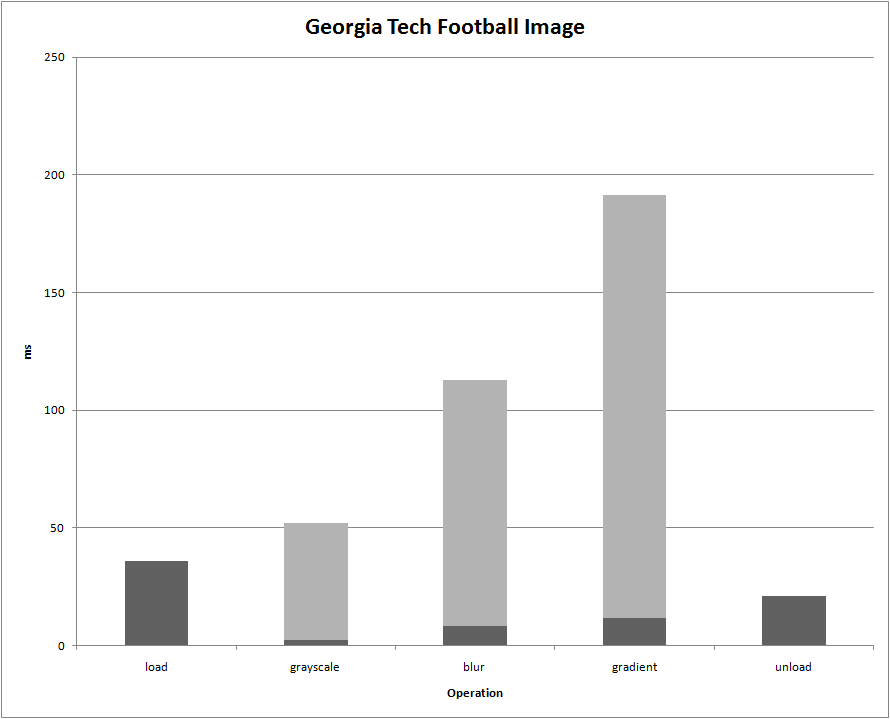
\includegraphics[scale=.35]{gtPerf.png}
\caption{OpenCV versus CUDA}
\label{fig}
\end{figure}
\begin{figure}[p]
\centering
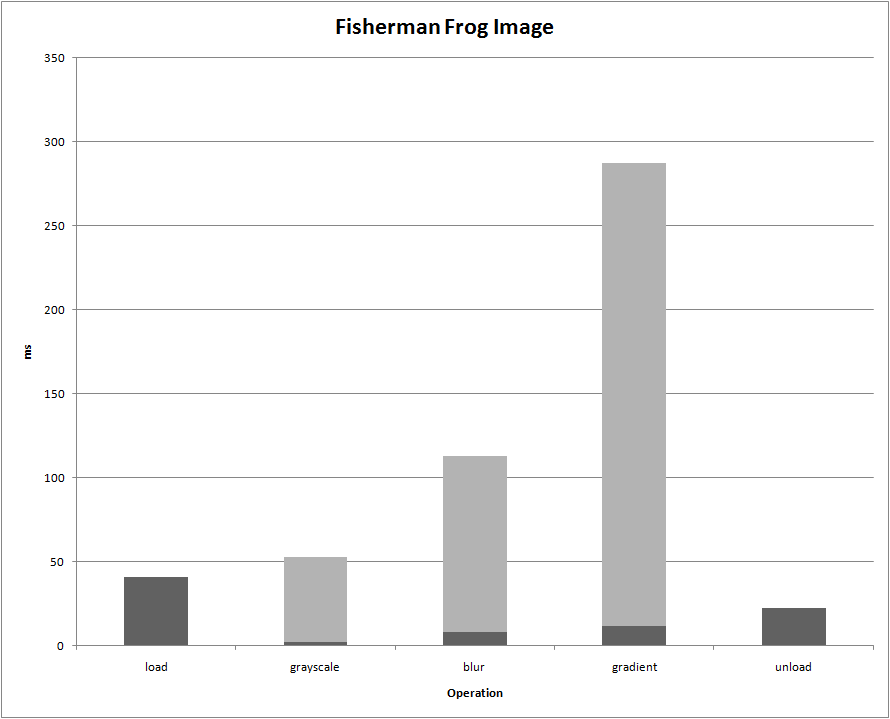
\includegraphics[scale=.35]{fisherFrogPerf.png}
\caption{OpenCV versus CUDA}
\label{fig}
\end{figure}
\begin{figure}[p]
\centering
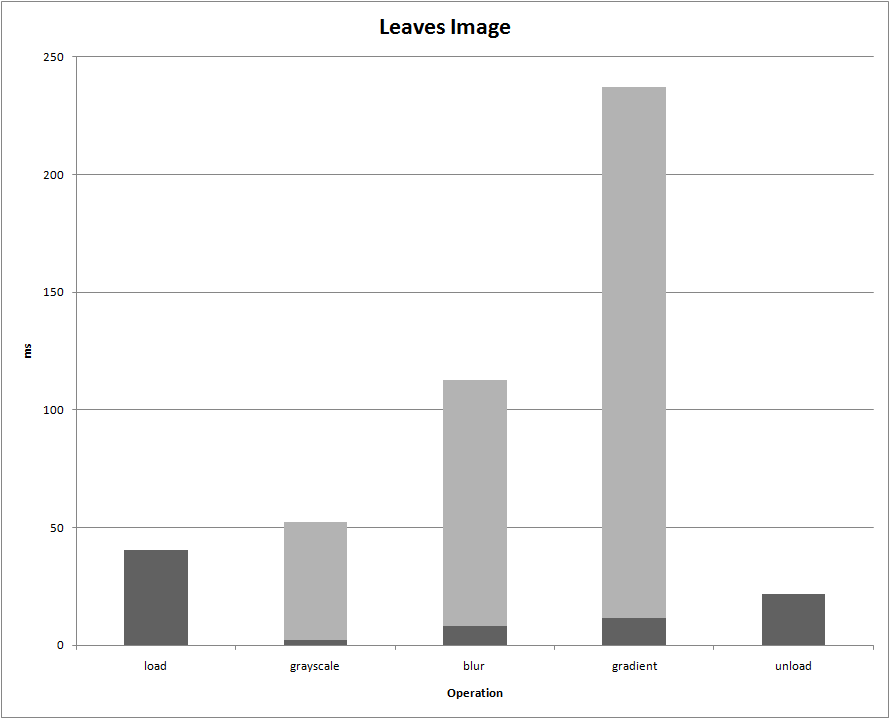
\includegraphics[scale=.35]{leavesPerf.png}
\caption{OpenCV versus CUDA}
\label{fig}
\end{figure}
\begin{figure}[p]
\centering
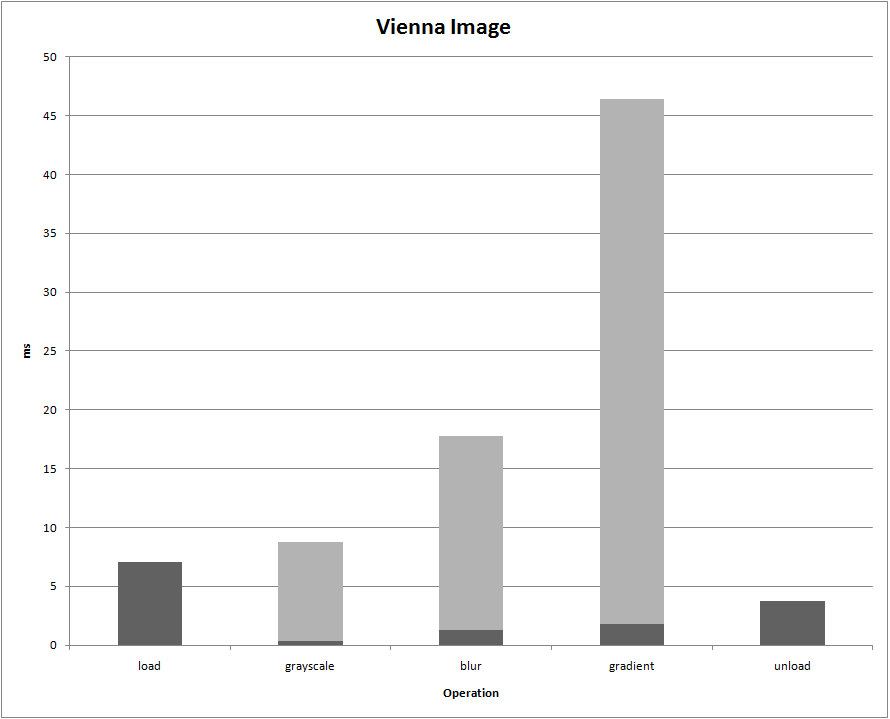
\includegraphics[scale=.35]{viennaPerf.png}
\caption{OpenCV versus CUDA}
\label{fig}
\end{figure}
\begin{figure}[p]
\centering
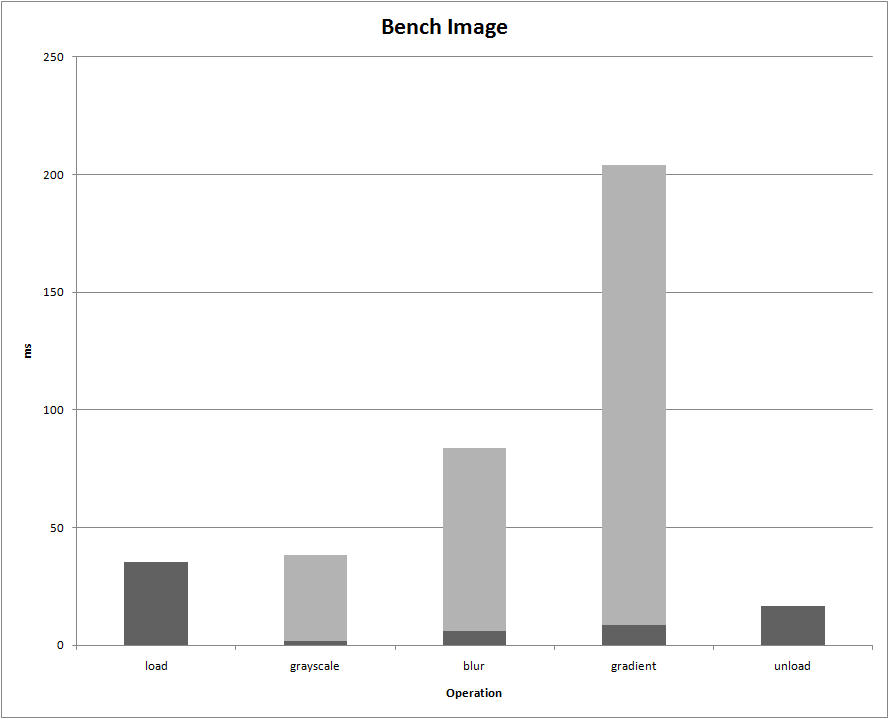
\includegraphics[scale=.35]{benchPerf.png}
\caption{OpenCV versus CUDA}
\label{fig}
\end{figure}

%fig. 1 - GT football
%fig. 2 monument
%fig. 3 fisherfrog
%fig. 4 leaves
%fig 5 vienna
%fig 6 wooden bench
%
%fig 7 cuda normalized perf
%fig 8 open cv normalized perf
%
%fig 9 gt fb
%fig 10 fisherfrog
%fig 11 leaves perf
%fig 12 vienna perf
%fig 13 wooden bench perf

Figures 1 and 2 present the performance results of the CUDA implementation and the OpenCV reference implementation.  The CUDA image conversions are each dominated by data transfers to load the original image and then unload the edge detected version.  The results of the load and unload operations show that the unload operation equals about 33\% of the load time.  This is because the original images are an RGB bitmap while the output is a gray scale image where each pixel represents a single byte as opposed to three.

The load and unload times required for CUDA is highly dependent on the bus architecture of the GPU card and whether the PCI Express lane is shared with other cards.  The test server provided on the Jinx cluster is described as having a PCI Express 2.0 16x interface.  From our research this card should support data transfers of 4000 MB/s.  Using the RGB fisherfrog image as an example, its size, s, of 36,636,726 bytes should require a minimum transfer time of s(3 bytes per pixel)/(4000)(1024)(1024), or 26 ms.  We observed the transfer to require 41 ms.

While each of our test images varied in size (with GT, fisherfrog, and leaves each consuming 35 MB and vienna consuming 5.5 MB) Figure 7 shows that each of the image processing operations performed at nearly a constant rate.  We believe this is due to the optimized nature of CUDA and its ability to efficiently perform SIMD operations. The OpenCV implementation results shown in Figure 8 highlight the lack of efficiency achieved with a single-threaded, CPU.  The variation observed in the rate of the gradient calculation.

The gradient calculation is somewhat dependent on the characteristics of the image.  The results of the Georgia Tech football helmet presented in Figure 9 shows the gradient operation requiring 180 ms vs. 276 ms for the fisherman frog image and 225 ms for the leaves image.  Clearly, the original football image in Figure 1 has fewer well-defined edges.  While cropped, the Georgia Tech football image resulted in very few edges from the background and foreground helmets.

\section{Future Considerations}

Our CUDA implementation lacks the additional processing found in each the OpenCV.  The images produced by OpenCV have well-defined lines since each of the edge points along the same gradient were also connected.

Performance could also be enhanced by merging two of the processing stages.  In our implementation, Gaussian blur and gradient detection are separate methods that require all CUDA threads to synchronize and copy data to a read only buffer before continuing.

The speed of CUDA processing could also permit pipelined operations where smaller images from a video feed to be processed in real-time.

\section{Summary}

The results clearly show the benefits of using CUDA or other general purpose GPU libraries. The level of parallelism in graphics devices is unmatched at present by any other consumer level hardware. However, with this high level of parallelism one also has to be prepared to encounter both algorithmic and optimization challenges. Graphics cards have a unique memory hierarchy and pipeline that many developers are unfamiliar with and there is a learning curve with the style of programming required by CUDA and other SIMD languages.

\section{References}

[1] Bill Green (2002). Canny Edge Detection Tutorial.  Retrieved November 9, 2011, from
sites.google.com/site/setiawanhadi2/1CannyEdgeDetectionTutorial.pdf

[2] Yuancheng �Mike� Luo and Ramani Duraiswami (2009). Canny Edge Detection on NVIDIA CUDA. Retrieved November 9, 2011, from http://www.cs.umd.edu/Honors/reports/luo\_08.pdf

[3] Canny, J., A Computational Approach To Edge Detection, IEEE Trans. Pattern Analysis and Machine Intelligence, 8(6):679�698, 1986

[5] PCI Express and PXI Express Bandwidth Demos, http://zone.ni.com/devzone/cda/tut/p/id/3768

\end{document}
